\documentclass[11pt, a4paper]{article}

\usepackage{array}
\usepackage[portuguese]{babel}
\usepackage{cite}
\usepackage{float}
\usepackage[a4paper, margin=2cm]{geometry}
\usepackage{graphicx}
\usepackage{hyperref}
\usepackage{longtable}

\chardef\_=`_

\title{
    \vspace*{\fill}
    \textbf{
        Sistemas Distribuídos -- Trabalho Prático  \\
        \large Base de dados concorrente com acesso remoto
    }
}
\author{
    \begin{tabular}{ll}
        Carolina Sofia Lopes Queirós Pereira  & A100836 \\
        Diogo Luís Barros Costa               & A100751 \\
        Humberto Gil Azevedo Sampaio Gomes    & A104348 \\
        Sara Azevedo Lopes                    & A104179
    \end{tabular}
}
\date{28 de dezembro de 2024 \vspace*{\fill}}

\begin{document}

% Use rsvg-convert instead of direct EPS to get font embedding
\immediate\write18{neato -Tsvg dot/Architecture.dot | rsvg-convert -f eps -o dot/Architecture.eps -}
\immediate\write18{plantuml -teps:text uml/sequence.uml}

\setlength{\parskip}{\baselineskip}
\setlength{\parindent}{0pt}

\begin{titlepage}
    \maketitle
\end{titlepage}

\pagenumbering{gobble}
\pagebreak
\pagenumbering{arabic}

\begin{abstract}
    O trabalho prático proposto consiste no desenvolvimento de uma base de dados que armazena, em
    memória, associações chave-valor. A base de dados é gerida por um servidor, que serve pedidos de
    clientes comunicados via TCP/IP, garantido a atomicidade das suas execuções. Desenvolveu-se uma
    solução concorrente, utilizando primitivas de sincronização baseadas em monitores. Procurou-se
    diminuir a contenção e minimizar o número de \emph{threads} acordadas, pelo que se implementaram
    diversas estratégias de controlo de concorrência, procurando-se aumentar o desempenho do
    \emph{software} sem sacrificar a sua correção. O desempenho destas várias estratégias foi
    medido com recurso a uma ferramenta de testes também desenvolvida, e os resultados dos
    \emph{benchmarks} realizados apresentam-se neste relatório.
\end{abstract}

\section{Arquitetura do programa}

O \emph{software} desenvolvido foi dividido em componentes, que se apresentam na figura abaixo,
juntamente com as dependências entre si:

\begin{minipage}{0.5\textwidth}
    \begin{figure}[H]
        \centering
        \includegraphics[width=\textwidth]{dot/Architecture.eps}
        \caption{Dependências entre os vários componentes da solução desenvolvida.}
        \label{architecture}
    \end{figure}
\end{minipage}
\hspace{0.03\textwidth}
\begin{minipage}{0.47\textwidth}
    \setlength{\parskip}{\baselineskip}
    \setlength{\parindent}{0pt}
    A maioria da funcionalidade do \emph{software} está localizada nas bibliotecas \texttt{common} e
    \texttt{libserver}:

    \begin{itemize}
        \item \texttt{common}
        \begin{itemize}
            \item Mensagens do protocolo de comunicação entre \texttt{client} e \texttt{server}, e a
                sua serialização e deserialização;

            \item Lógica de comunicação do cliente.
        \end{itemize}

        \item \texttt{libserver}
        \begin{itemize}
            \item Várias implementações da estrutura de armazenamento de dados (\emph{backends}),
                com estratégias de controlo de concorrência distintas.

            \item Lógica de comunicação do servidor.
        \end{itemize}
    \end{itemize}
\end{minipage}

Os programas \texttt{client} e \texttt{server} não passam de \emph{wrappers} à volta das bibliotecas
\texttt{common} e \texttt{libserver}, respetivamente. No programa \texttt{tester}, é implementada
uma \emph{framework} para \emph{benchmarking} tanto dos \emph{backends} em \texttt{libserver} como
da base de dados completa.

\section{\emph{Backends} implementados}

\subsection{\texttt{SimpleHashMapBackend}}

Este \emph{backend} consiste numa tabela de \emph{hash} que armazena as associações, e cujo acesso
concorrente é moderado por um \emph{lock} de leitores e escritores. Há também duas variáveis de
condição (associadas ao \emph{lock} de escritores), uma notificada quando os conteúdos da base de
dados são alterados, e outra quando todas as operações \texttt{getWhen} terminam de verificar se a
sua condição é verdadeira.

A operação \texttt{getWhen} é a mais complexa: após adquirir o \emph{lock} para escritas, regista-se
a \emph{thread} atual como estando à espera de uma atualização, e espera-se na variável de condição
associada a atualizações da base de dados. As operações \texttt{put} e \texttt{multiPut}, quando
terminam, sinalizam as \emph{threads} à espera desta variável de condição (caso as haja). As
\emph{threads} na operação \texttt{getWhen} podem, caso se verifique a sua condição, remover-se da
lista de \emph{threads} à espera e devolver um valor. Quando a última \emph{thread} a executar um
\texttt{getWhen} verifica a sua condição, sinaliza as \emph{threads} à espera do fim da execução das
operações \texttt{getWhen} (\emph{threads} no início das operações \texttt{put} e \texttt{multiPut}).

\subsection{\texttt{MultiConditionHashMapBackend}}

Este \emph{backend} é muito semelhante ao anterior, com a diferença de que são utilizadas mais
variáveis de condição relativas à alteração da base de dados, para uma maior granularidade na
sinalização de \emph{threads}. As operações \texttt{getWhen}, no seu início, criam, caso não exista,
uma variável de condição associada à atualização da sua chave, pela qual esperam, e as operações
\texttt{put} e \texttt{multiPut} sinalizam apenas as \emph{threads} à espera de variáveis de
condição associadas às chaves modificadas. A execução de uma operação \texttt{getWhen} também exige
a destruição de uma variável de condição caso não haja mais \emph{threads} dela dependentes.

Uma abordagem alternativa que evita a criação de novas variáveis de condição foi considerada. Esta
envolve a criação inicial de $N$ variáveis de condição, às quais as chaves se associam pela sua
\emph{hash}. No entanto, testes empíricos demonstraram que esta solução apresenta um desempenho
semelhante à abordagem com criação de novas variáveis de condição, não se justificando alterações ao
\emph{backend}.

\subsection{\texttt{ShardedHashMapBackend}}

Este \emph{backend} consiste no uso de $N$ tabelas de \emph{hash} (\emph{shards}), associadas a $N$
\emph{locks} de leitores e escritores. A \emph{hash} de uma chave determina o \emph{shard} onde será
armazenada. As operações \texttt{get} e \texttt{put} precisam de adquirir apenas um \emph{lock}, e
as operações \texttt{multiGet} e \texttt{multiPut} precisam de adquirir vários \emph{locks},
fazendo-o ordenadamente para evitar \emph{deadlocks}, e usado \emph{two-phase locking} para diminuir
o tempo que cada \emph{lock} se encontra adquirido.

Não foi possível implementar a operação \texttt{getWhen} neste \emph{backend} sem prejudicar
gravemente o seu desempenho, pelo que esta não foi implementada. Uma operação de escrita precisa de
garantir que nada é escrito na base de dados que influencie o resultado das operações
\texttt{getWhen} a processar, podendo fazê-lo com a aquisição dos \emph{locks} associados aos
\emph{shards} das chaves necessárias. No entanto, para conhecer os \emph{locks} que deve adquirir,
teria, em primeiro lugar, de adquirir os \emph{locks} associados às chaves a escrever, e adquirir
outros \emph{locks} posteriormente poderia causar a violação da ordenação da aquisição de
\emph{locks}, conduzindo a uma possível situação de \emph{deadlock}. Este problema poderia ter sido
resolvido com um \emph{lock} ao nível da coleção, mas testes empíricos mostraram que o seu uso fazia
com que este \emph{backend} tivesse um desempenho semelhante aos \emph{backends} de \emph{lock}
único apresentados.

\section{Arquiteturas do cliente e do servidor}

Na figura abaixo, observa-se uma representação das arquiteturas do cliente e do servidor da base de
dados. No cliente, o envio de uma mensagem é feito por qualquer \emph{thread} da aplicação, através
de uma escrita no \emph{socket}, cujo acesso é moderado por um \emph{lock}. Há uma \emph{thread}
dedicada à exclusivamente à leitura de mensagens do servidor e à sua deserialização. Após um pedido,
as \emph{threads} da aplicação bloqueiam numa variável de condição até obterem uma resposta do
servidor, que é sinalizada pela \emph{thread} de receção de mensagens. Para diminuir o número de
\emph{threads} sinalizadas, são inicialmente criadas várias variáveis de condição, e uma
\emph{thread} escolhe a variável de condição onde bloquear de acordo com o identificador da mensagem
enviada.

Quanto ao servidor, uma \emph{thread} em cada conexão é responsável por deserializar os pedidos do
cliente e despachá-los para uma \emph{thread pool}, que os executa. A \emph{thread pool}
implementada regula o seu número de \emph{threads} para se ajustar ao volume de pedidos dos
clientes. As \emph{threads} da \emph{thread pool}, após terminarem as operações na base de dados,
respondem aos clientes, escrevendo em \emph{buffers} de mensagens, que são lidos por \emph{threads}
de cada conexão, responsáveis apenas por escritas nos \emph{sockets}. Deste modo, é possível que o o
resultado de um pedido de um cliente seja difundido por vários clientes, sem que clientes lentos
bloqueiem a \emph{thread} na \emph{thread pool}. De momento, nenhum \emph{backend} tira proveito
desta funcionalidade.

\begin{figure}[H]
    \centering
    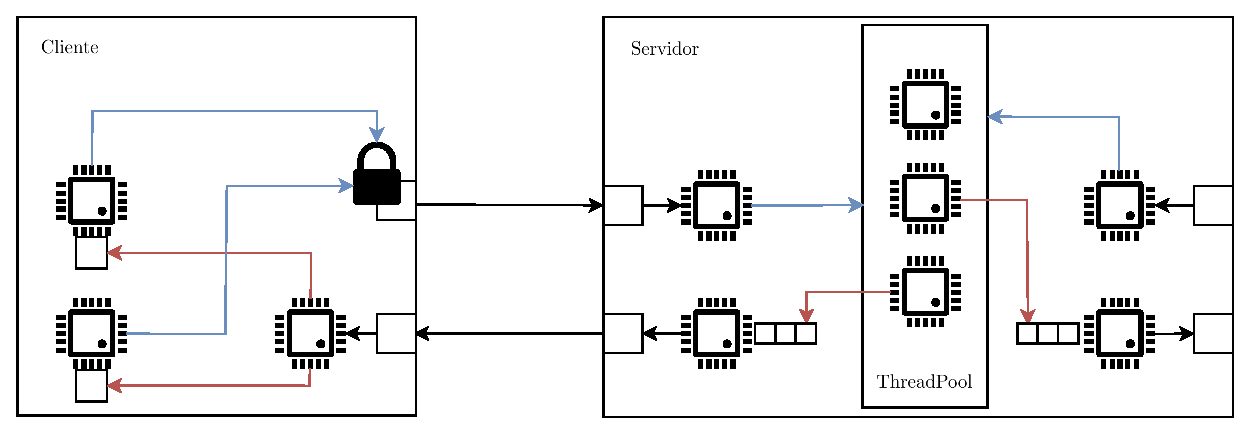
\includegraphics[width=\textwidth]{res/ClientServer.eps}
    \caption{Arquiteturas \emph{multi-thread} do cliente e do servidor.}
    \label{client-server-architecture}
\end{figure}

\section{Protocolo de comunicação entre um cliente e o servidor}

\begin{minipage}{0.5\textwidth}
    \setlength{\parskip}{\baselineskip}
    \setlength{\parindent}{0pt}

    À direita, apresenta-se um diagrama de sequência de uma possível troca de mensagens entre um
    cliente e o servidor. Não são representados segmentos da camada de transporte (TCP).

    As duas primeiras mensagens permitem a autenticação do cliente: o cliente pede a sua
    autenticação / registo, e espera que o servidor responda (a autorizar o cliente ou a reportar um
    erro).

    As restantes mensagens correspondem a pedidos do cliente para realizar operações na base de
    dados, e às respostas do servidor, pelas quais o cliente aguarda. É de notar que todos os
    pedidos se encontram numerados (campo \texttt{id}), e é possível que o servidor envie respostas
    numa ordem diferente da qual recebeu os pedidos (campo \texttt{requestId}), permitindo a
    existência de clientes \emph{multi-threaded}. Outra nota a fazer é que certas mensagens são
    utilizadas para vários propósitos. Por exemplo, são utilizadas mensagens do tipo
    \texttt{GetResponseMessage} para responder tanto a pedidos \texttt{get} como \texttt{getWhen},
    uma vez que o conteúdo da resposta é o mesmo.
\end{minipage}
\hspace{0.03\textwidth}
\begin{minipage}{0.47\textwidth}
    \begin{figure}[H]
        \centering
        \includegraphics[width=\textwidth]{uml/sequence.eps}
        \caption{Diagrama de sequência da troca de mensagens entre um cliente e o servidor.}
        \label{sequence}
    \end{figure}
\end{minipage}

A serialização é feita com recurso às classes \texttt{Data[Input|Output]Stream}. Devido à natureza
multi-plataforma da linguagem Java, é possível a execução do cliente em diversos sistemas. Ademais,
devido à documentação publicamente disponível das classes mencionadas, também é possível interagir
com o servidor utilizando outras tecnologias (ex.: C).

\section{\emph{Framework} de testes}

\subsection{Funcionalidade e implementação}

Foi desenvolvida uma \emph{framework} para testes de desempenho da base de dados. Um teste de
desempenho começa com a criação de uma base de dados e um povoamento inicial. Depois, são criadas
várias \emph{threads}, e cada uma gera operações de leitura e escrita aleatoriamente, executando-as
e medindo o tempo de execução de cada uma. Estes tempos são utilizados para o cálculo da média e do
desvio padrão do tempo de execução de cada tipo de operação. O número total de operações a executar
é dividido em blocos, que são dinamicamente distribuídos pelas \emph{threads}. O teste termina
quando o número o conjunto de \emph{threads} completa um número predeterminado de operações.

A principal dificuldade na implementação da \emph{framework} relacionou-se com a operação
\texttt{getWhen}, que bloqueia até uma condição se verificar na base de dados. É possível que todas
as \emph{threads} bloqueiem, e não haja nenhuma \emph{thread} disponível para desbloquear as
\emph{threads} bloqueadas. Para resolver este problema, é criada uma \emph{thread} no início de cada
teste, responsável por desbloquear \emph{threads} bloqueadas em operações \texttt{getWhen}. Antes de
uma \emph{thread} executar uma operação \texttt{getWhen}, atualiza uma variável que armazena a
condição na qual irá bloquear. A \emph{thread} de desbloqueio itera constantemente por estas
condições, atualizando a base de dados de modo a desbloquear outras \emph{threads}. Assim, não faz
sentido que a \emph{framework} de testes meça o tempo médio de execução de operações
\texttt{getWhen}, visto que este está altamente dependente de quando a \emph{thread} de desbloqueio
é escalonada, refletindo fracamente o desempenho da base de dados.

Outra possibilidade de resolução deste problema menos computacionalmente intensiva consiste na
existência de uma (ou várias) \emph{threads} responsáveis pela geração das operações, que garantem
que todas as operações \texttt{getWhen} são correspondidas por uma operação de escrita posterior que
desbloqueia a \emph{thread} a executar o \texttt{getWhen}. No entanto, esta estratégia pode exigir o
uso de blocos muito pequenos para assegurar que uma dada fração das operações sejam do tipo
\texttt{getWhen}, aumentando o \emph{overhead} do controlo de concorrência, e possivelmente
impedindo a \emph{framework} de testes de medir o desempenho máximo da base de dados.

Por último, foram três as bibliotecas utilizadas para auxiliar o desenvolvimento da \emph{framework}
de testes. Para implementações de distribuições numéricas (uniforme, Zipf, \ldots), a biblioteca
Apache Commons Math \cite{apache-commons-math} foi utilizada, e as bibliotecas JFreeChart
\cite{jfreechart} e Apache XML Graphics \cite{apache-xml-graphics} foram utilizadas para a geração
automática dos gráficos apresentados neste documento.

\subsection{Metodologia de testagem e resultados}

Procurou-se testar o desempenho da base de dados desenvolvida em diversos cenários. Para isso,
tirou-se proveito do elevadíssimo grau de configurabilidade da \emph{framework} de testes
desenvolvida, e foram concebidos diferentes \emph{benchmarks}, descritos no anexo
\ref{benckmark-description}, e executados num ambiente de execução descrito no anexo
\ref{hardware-software-description}. Testaram-se os \emph{backends} implementados diretamente, uma
vez que a comunicação cliente-servidor apenas adiciona um tempo aproximadamente constante a cada
medição, nada revelando e dificultando a comparação entre os \emph{backends}.

Abaixo, observam-se os tempos médios de execução das operações envolvidas no \emph{benchmark}
"Maioritariamente leituras"{}. Para qualquer operação e número de \emph{threads}, o desempenho dos
\emph{backends} de \emph{lock} único é aproximadamente igual, visto que o \emph{overhead} do
controlo de concorrência é o mesmo (aquisição de um \emph{lock} de escrita / leitura conforme a
operação). No entanto, o mesmo não é verdade para o \texttt{ShardedHashMapBackend}. Com uma
\emph{thread}, a necessidade de aquisição de vários \emph{locks} em operações \texttt{multiPut}
resulta num maior tempo de execução de cada operação. No entanto, com o aumento do número de
\emph{threads}, a granularidade dos \emph{locks} reduz a contenção, permitindo que as operações de
todos os tipos sejam menos demoradas. Neste \emph{backend}, a partir de 4 \emph{threads}, para
operações \texttt{multiGet}, o \emph{overhead} de controlo de concorrência é compensado pela menor
contenção.

\begin{longtable}{m{0.30\textwidth}m{0.30\textwidth}m{0.30\textwidth}}
    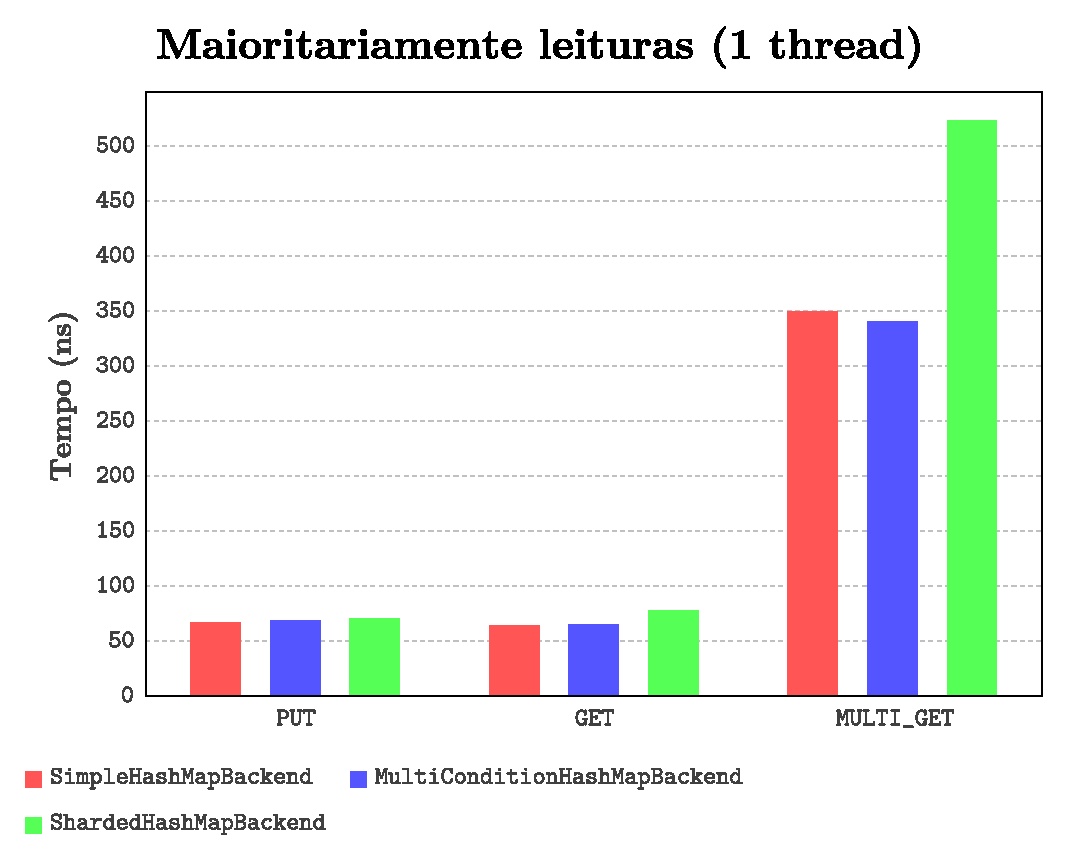
\includegraphics[width=0.30\textwidth]{autogen/Maioritariamente_leituras_1_thread.eps} &
    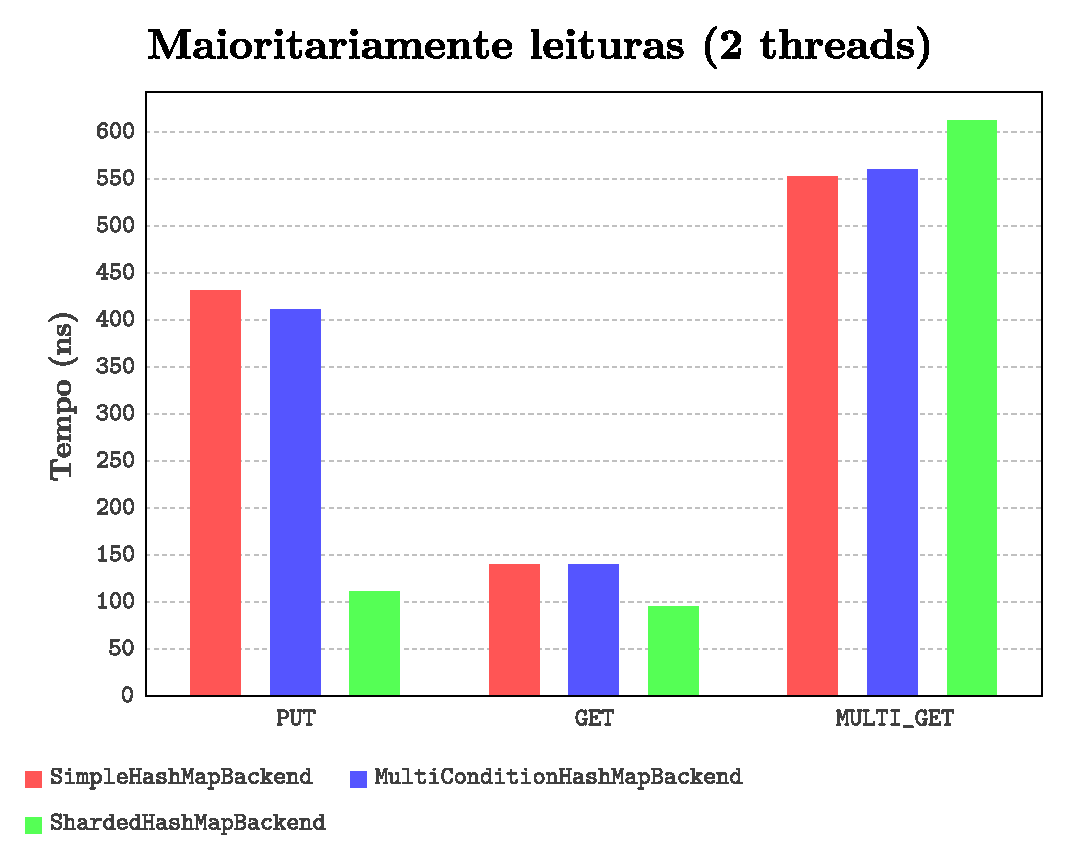
\includegraphics[width=0.30\textwidth]{autogen/Maioritariamente_leituras_2_threads.eps} &
    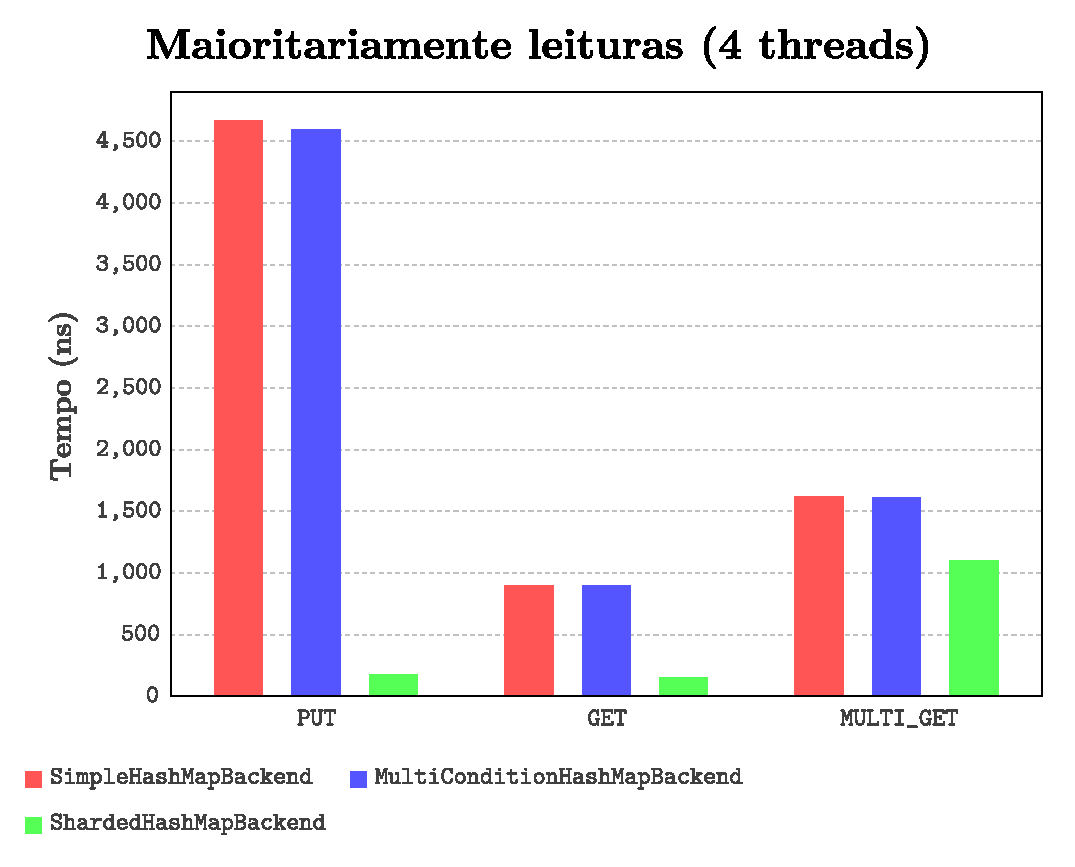
\includegraphics[width=0.30\textwidth]{autogen/Maioritariamente_leituras_4_threads.eps} \\
    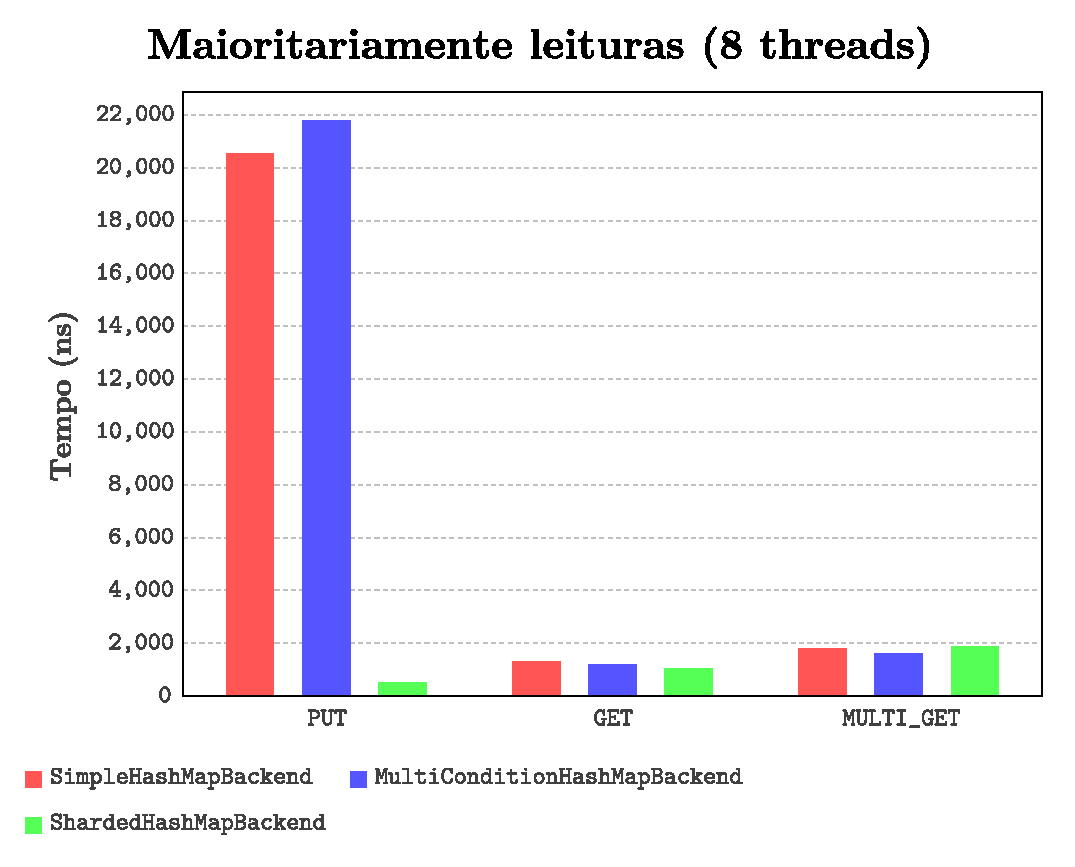
\includegraphics[width=0.30\textwidth]{autogen/Maioritariamente_leituras_8_threads.eps} &
    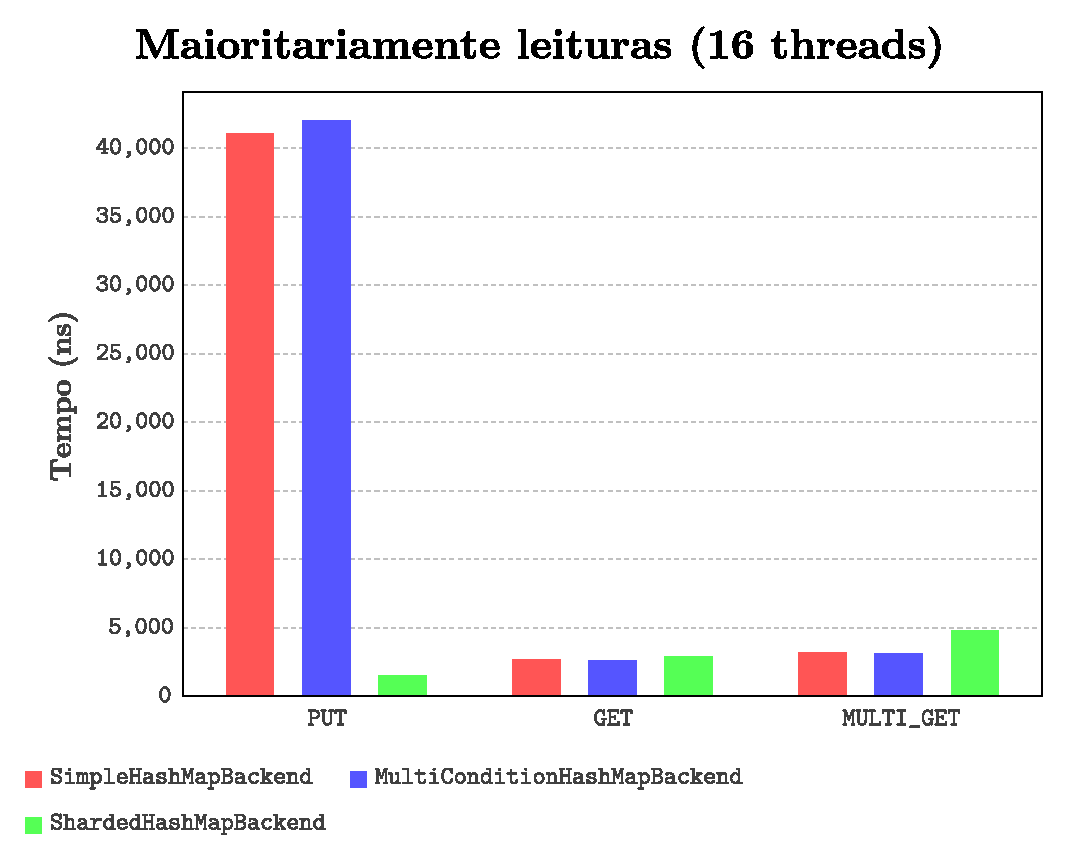
\includegraphics[width=0.30\textwidth]{autogen/Maioritariamente_leituras_16_threads.eps} &
    \stepcounter{figure}Figura \thefigure:
        Tempos médios de execução das diversas operações nos diversos \emph{backends}, para o
        \emph{benchmark} "Maioritariamente leituras"{}.
\end{longtable}

No \emph{benchmark} "Equilibrado"{}, a situação é semelhante à anterior. O
\texttt{ShardedHashMapBackend} apresenta um maior \emph{overhead} no controlo de concorrência em
operações que envolvem várias chaves, mas que é compensado por uma menor contenção quando uma
segunda \emph{thread} é introduzida. A partir de quatro \emph{threads}, nos \emph{backends} de
\emph{lock} único, observa-se que as operações \texttt{get} são mais demoradas que as \texttt{put}.
Isto deve-se à injustiça dos \emph{locks} de leitura e escrita utilizados que, em combinação com uma
maior competição entre leituras e escritas, dificulta que várias operações de leitura sejam
executadas em paralelo. Configurar estes \emph{locks} como justos elimina esta discrepância entre
leituras e escritas, mas origina tempos de execução cerca de três vezes maiores para ambas as
operações, pelo que se optou por manter os \emph{locks} injustos na implementação dos
\emph{backends}.

\begin{longtable}{m{0.30\textwidth}m{0.30\textwidth}m{0.30\textwidth}}
    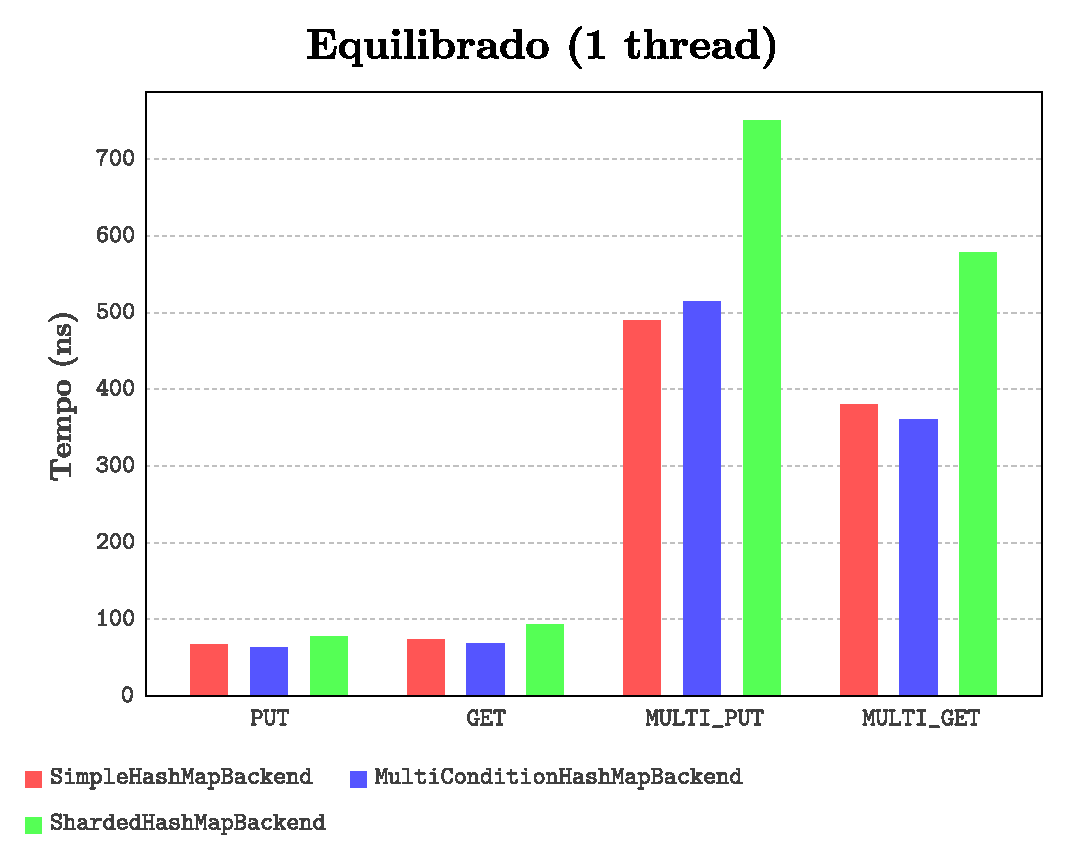
\includegraphics[width=0.30\textwidth]{autogen/Equilibrado_1_thread.eps} &
    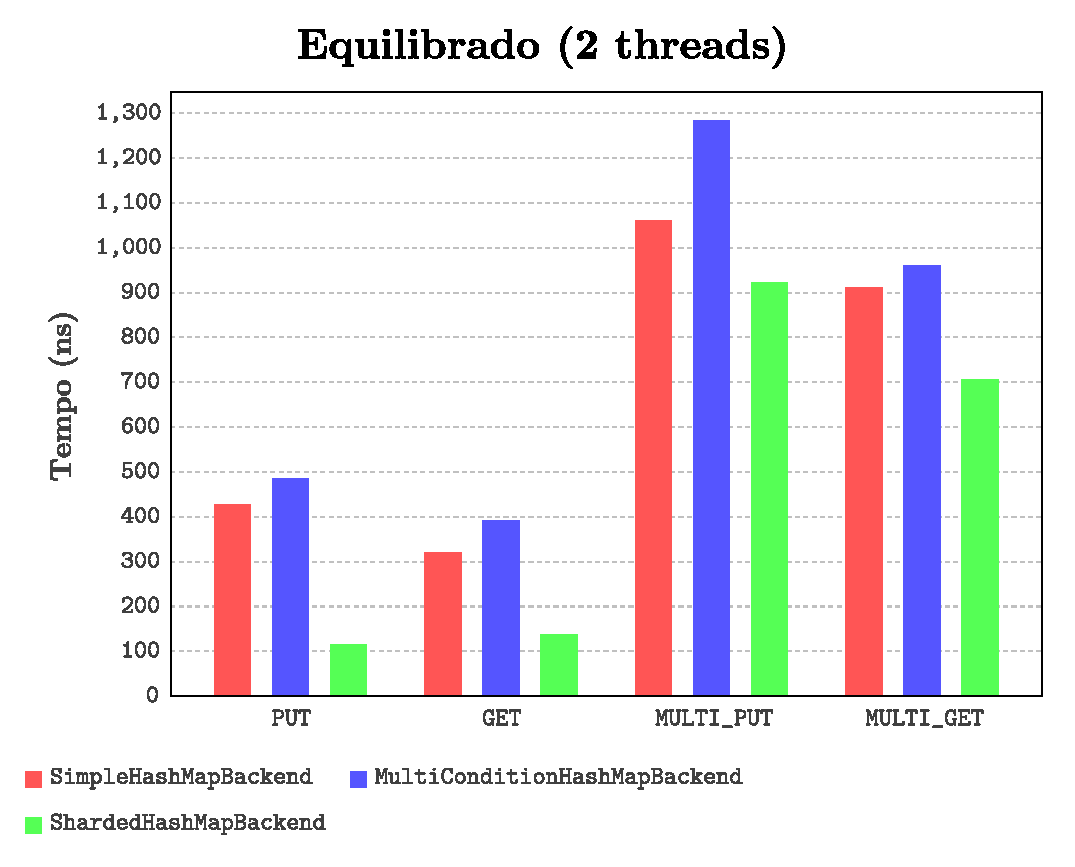
\includegraphics[width=0.30\textwidth]{autogen/Equilibrado_2_threads.eps} &
    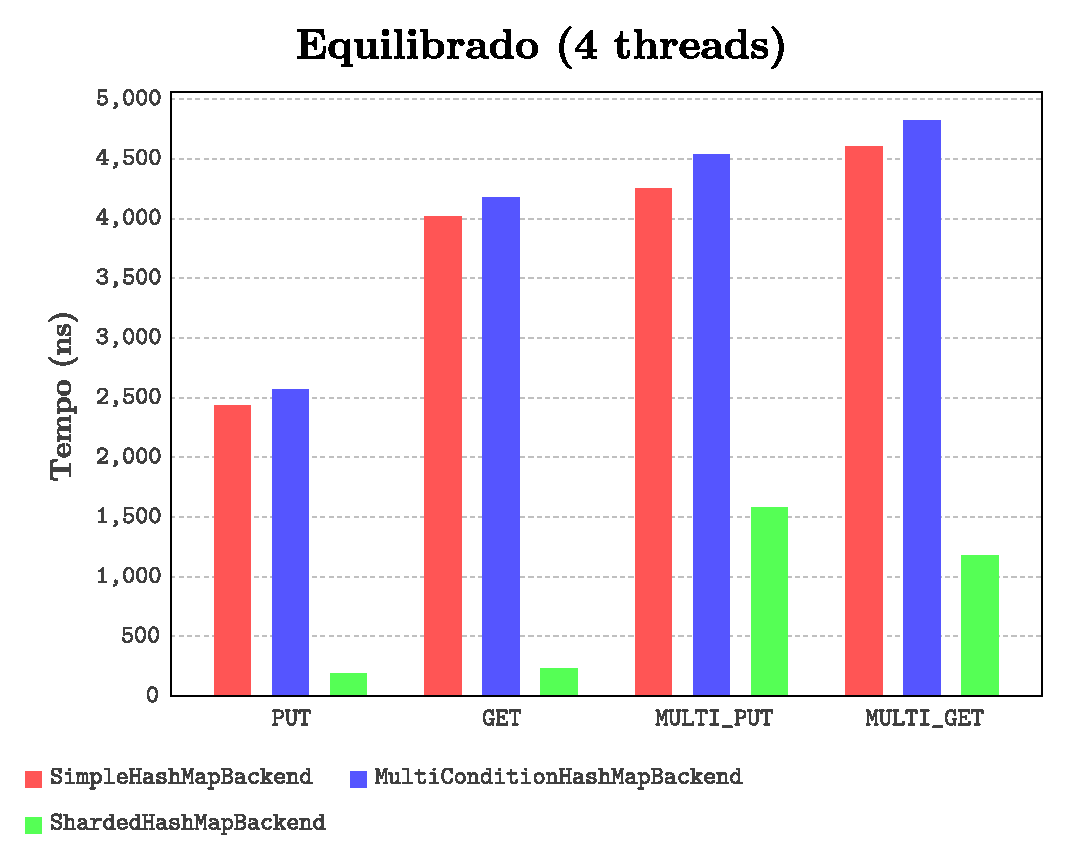
\includegraphics[width=0.30\textwidth]{autogen/Equilibrado_4_threads.eps} \\
    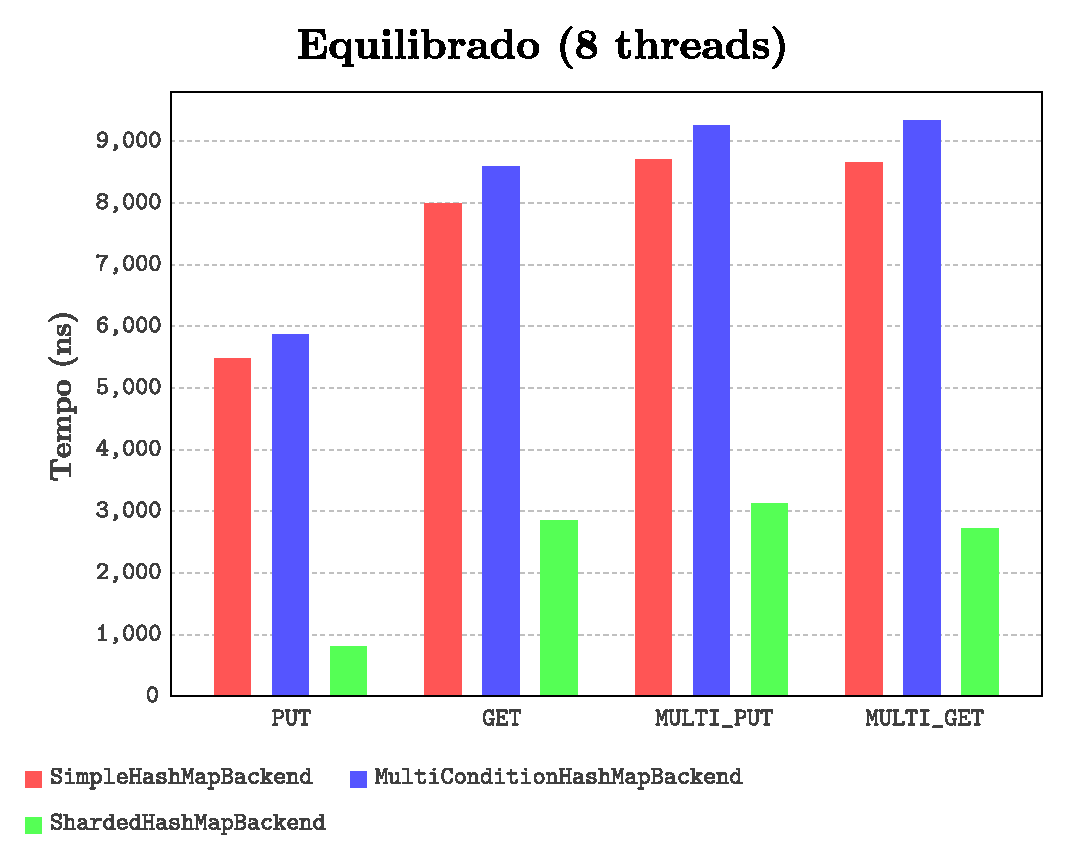
\includegraphics[width=0.30\textwidth]{autogen/Equilibrado_8_threads.eps} &
    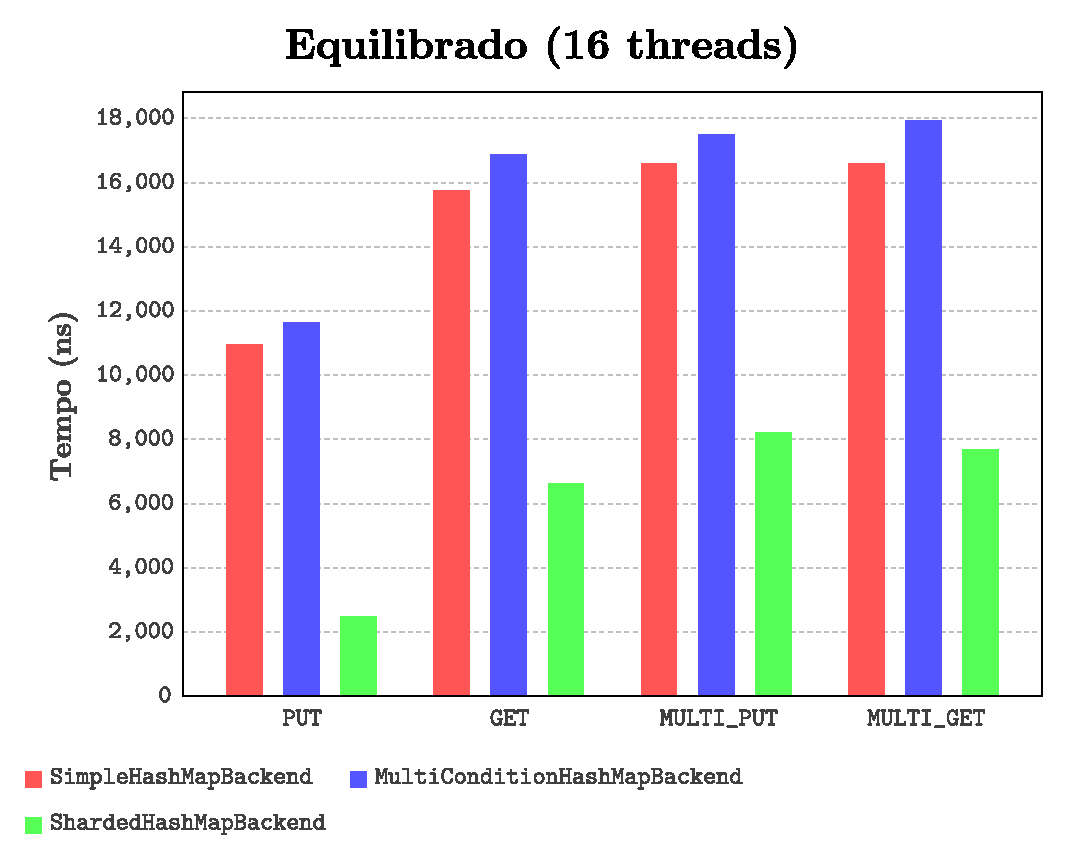
\includegraphics[width=0.30\textwidth]{autogen/Equilibrado_16_threads.eps} &
    \stepcounter{figure}Figura \thefigure:
        Tempos médios de execução das diversas operações nos diversos \emph{backends}, para o
        \emph{benchmark} "Equilibrado"{}.
\end{longtable}

Como mostram os gráficos abaixo, quando são executadas operações \texttt{getWhen} em duas
\emph{threads} ou menos, os \emph{backends} de \emph{lock} único apresentam sensivelmente o mesmo
desempenho, visto que o maior \emph{overhead} do controlo de concorrência do último \emph{backend}
nega as suas vantagens. No entanto, quando o número de \emph{threads} aumenta, o uso de variáveis de
condição de maior granularidade diminui o tempo de execução das operações de escrita, visto que
estas devem aguardar pelo término da execução dos \emph{triggers} (verificações de condições de
operações \texttt{getWhen}), e estes surgem em menor número. Também se observam melhorias, embora
menores, nos tempos das operações de leitura, visto que o menor número de \emph{triggers} a executar
faz com que o \emph{lock} para leitura possa ser adquirido, em média, mais rapidamente.

\begin{longtable}{m{0.30\textwidth}m{0.30\textwidth}m{0.30\textwidth}}
    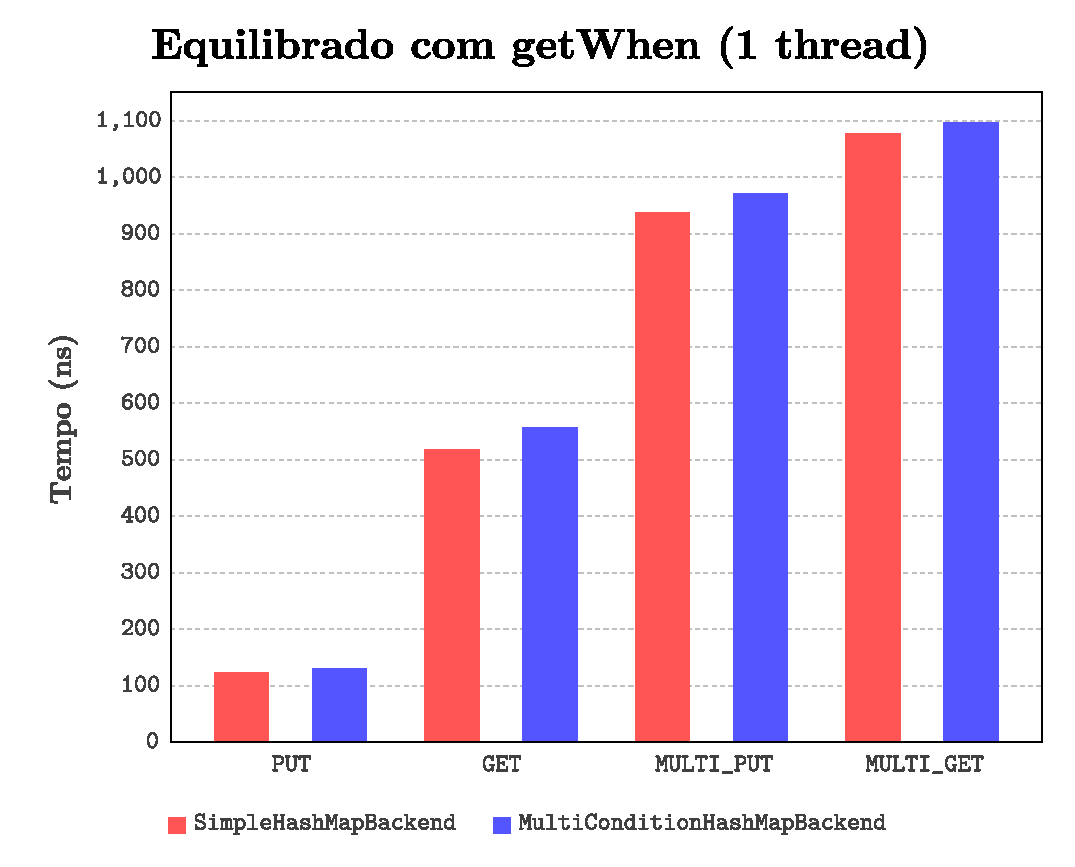
\includegraphics[width=0.30\textwidth]{autogen/Equilibrado_com_getWhen_1_thread.eps} &
    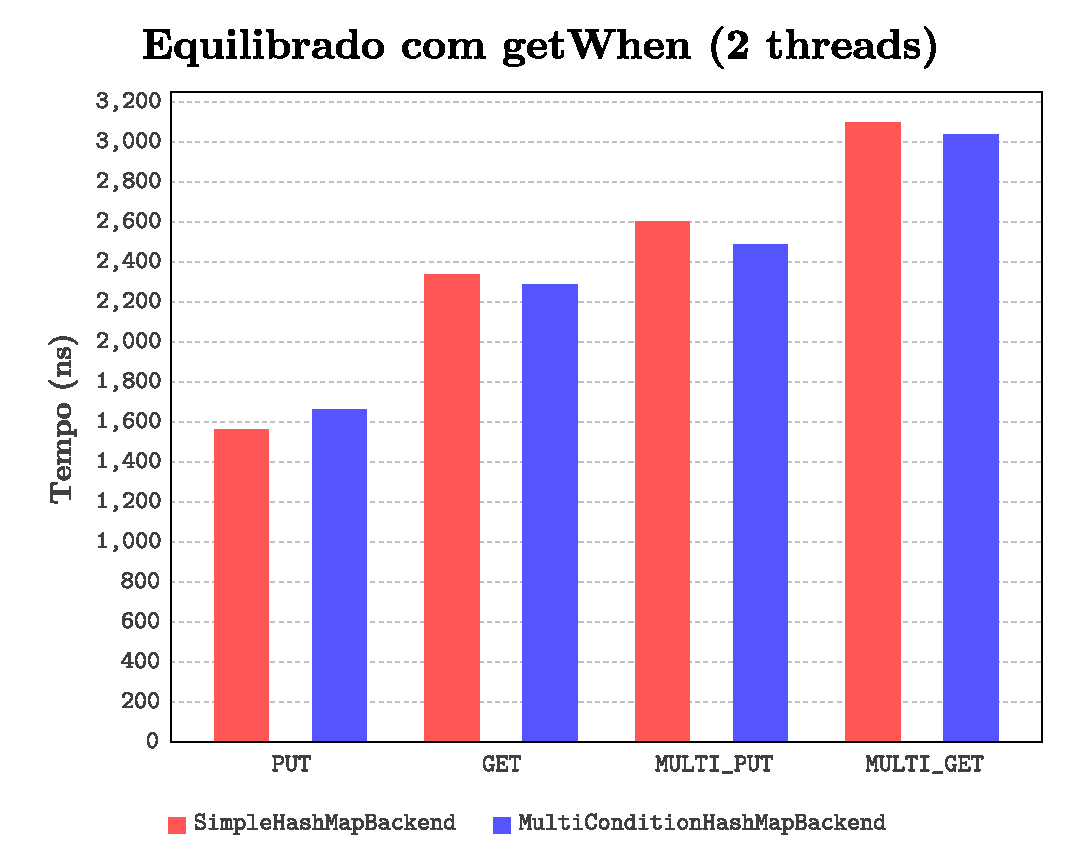
\includegraphics[width=0.30\textwidth]{autogen/Equilibrado_com_getWhen_2_threads.eps} &
    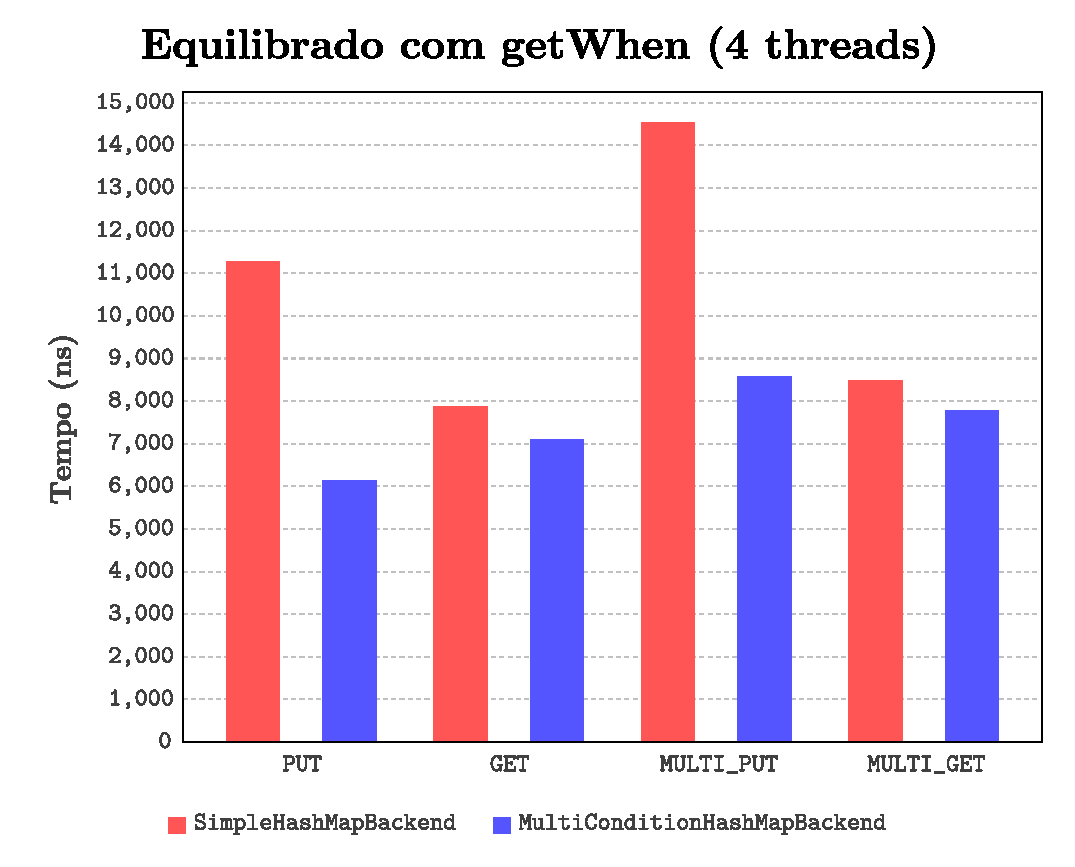
\includegraphics[width=0.30\textwidth]{autogen/Equilibrado_com_getWhen_4_threads.eps} \\
    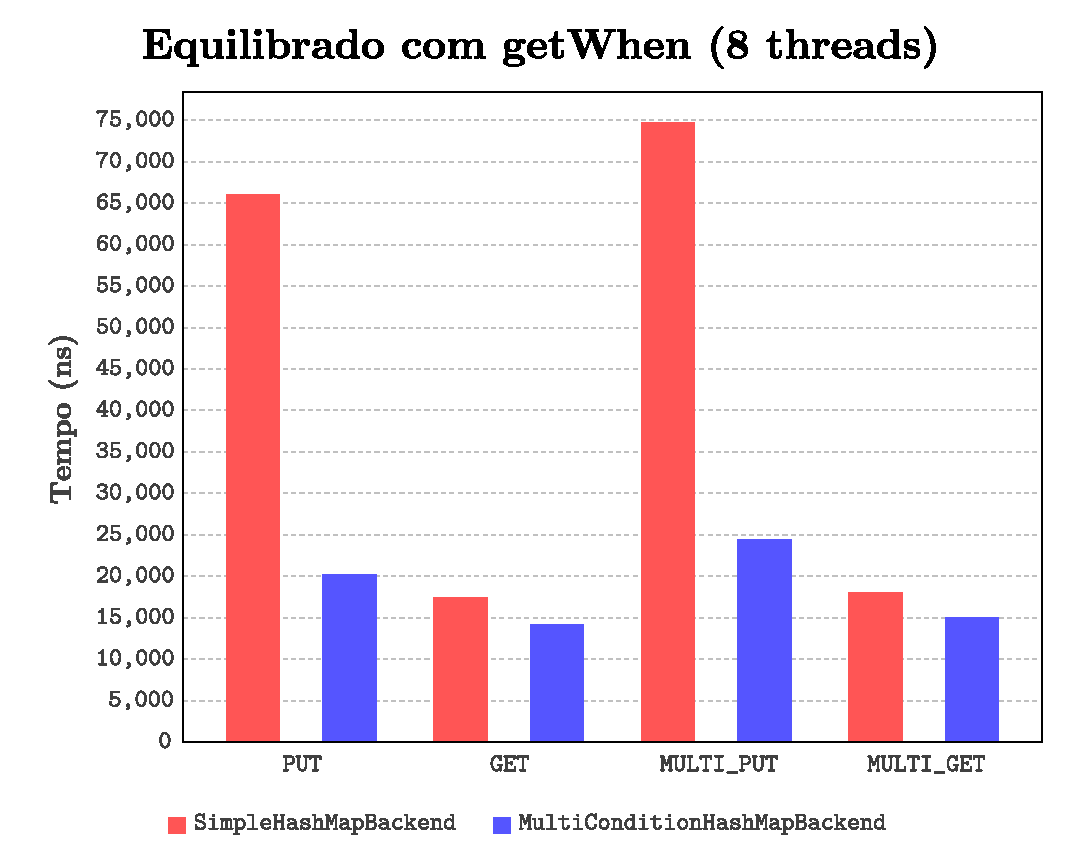
\includegraphics[width=0.30\textwidth]{autogen/Equilibrado_com_getWhen_8_threads.eps} &
    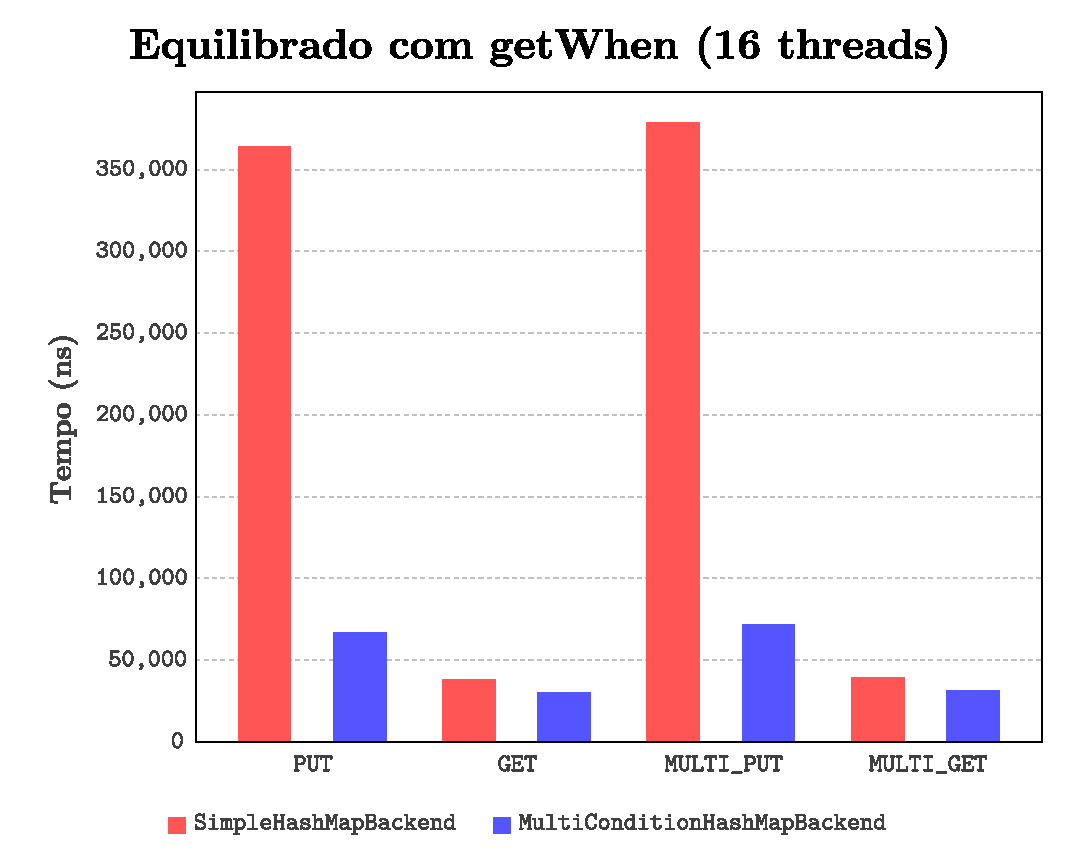
\includegraphics[width=0.30\textwidth]{autogen/Equilibrado_com_getWhen_16_threads.eps} &
    \stepcounter{figure}Figura \thefigure:
        Tempos médios de execução das diversas operações nos \emph{backends} que suportam operações
        \texttt{getWhen}, para o \emph{benchmark} "Equilibrado com getWhen"{}.
\end{longtable}

Como esperado, e como se observa nos gráficos acima, o tempo médio de cada operação aumenta com o
número de \emph{threads}, visto que cada \emph{thread} fica bloqueada em \emph{locks} por mais
tempo. No entanto, o que se procura avaliar é o desempenho total de um \emph{backend}, influenciado
tanto pelo número de \emph{threads} como pela duração de cada operação. Logo, apresenta-se abaixo a
duração de cada teste de acordo com as variáveis que a influenciam. Com a introdução de uma segunda
\emph{thread}, nos \emph{backends} de \emph{lock} único, apenas se verificam melhorias de desempenho
no \emph{benchmark} "Maioritariamente leituras"{}, visto que estas podem ocorrer em paralelo nestes
\emph{backends}, mas o mesmo já não é verdade para escritas. Com o \texttt{ShardedHashMapBackend},
como as operações de escrita realizadas não exigem a aquisição de um \emph{lock} sobre a totalidade
da base de dados, o melhor desempenho obtém-se para 4 \emph{threads} em ambos os \emph{benchmarks}.
A partir de 4 / 8 \emph{threads}, observa-se, de um modo geral, degradação do desempenho, uma vez
que é a partir deste ponto que se torna impossível haver afinidade das \emph{threads} de
\emph{software} às \emph{threads} físicas do processador utilizado, sendo o desempenho prejudicado
pelo tempo de sucessivas trocas de contexto.

\begin{figure}[H]
    \centering
    \begin{longtable}{m{0.45\textwidth}m{0.45\textwidth}}
        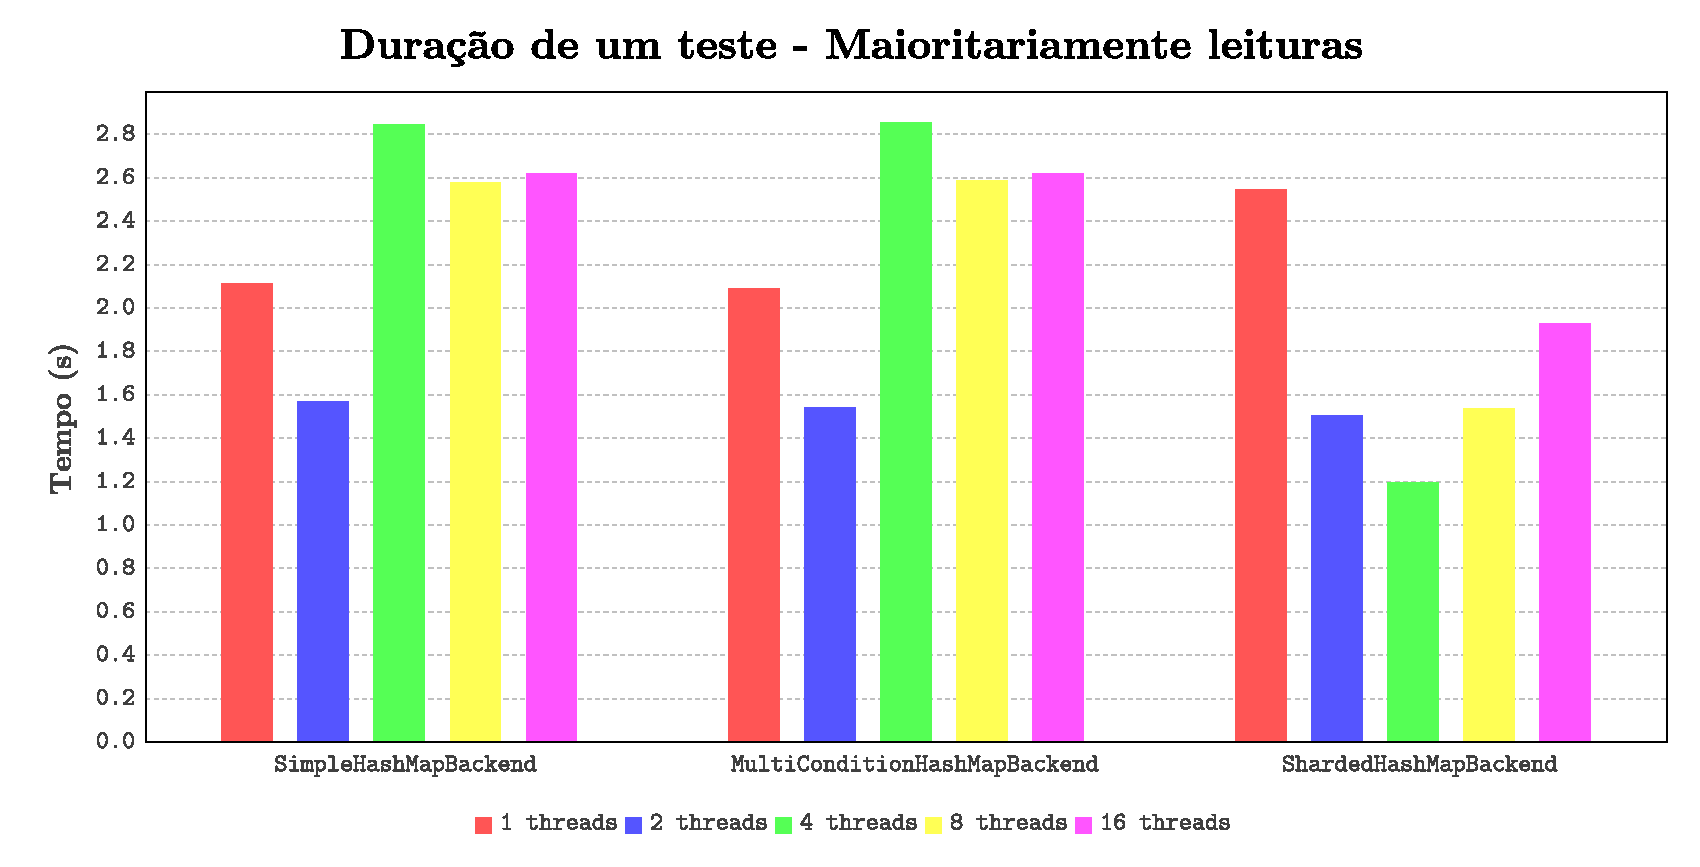
\includegraphics[width=0.45\textwidth]{autogen/Maioritariamente_leituras.eps} &
        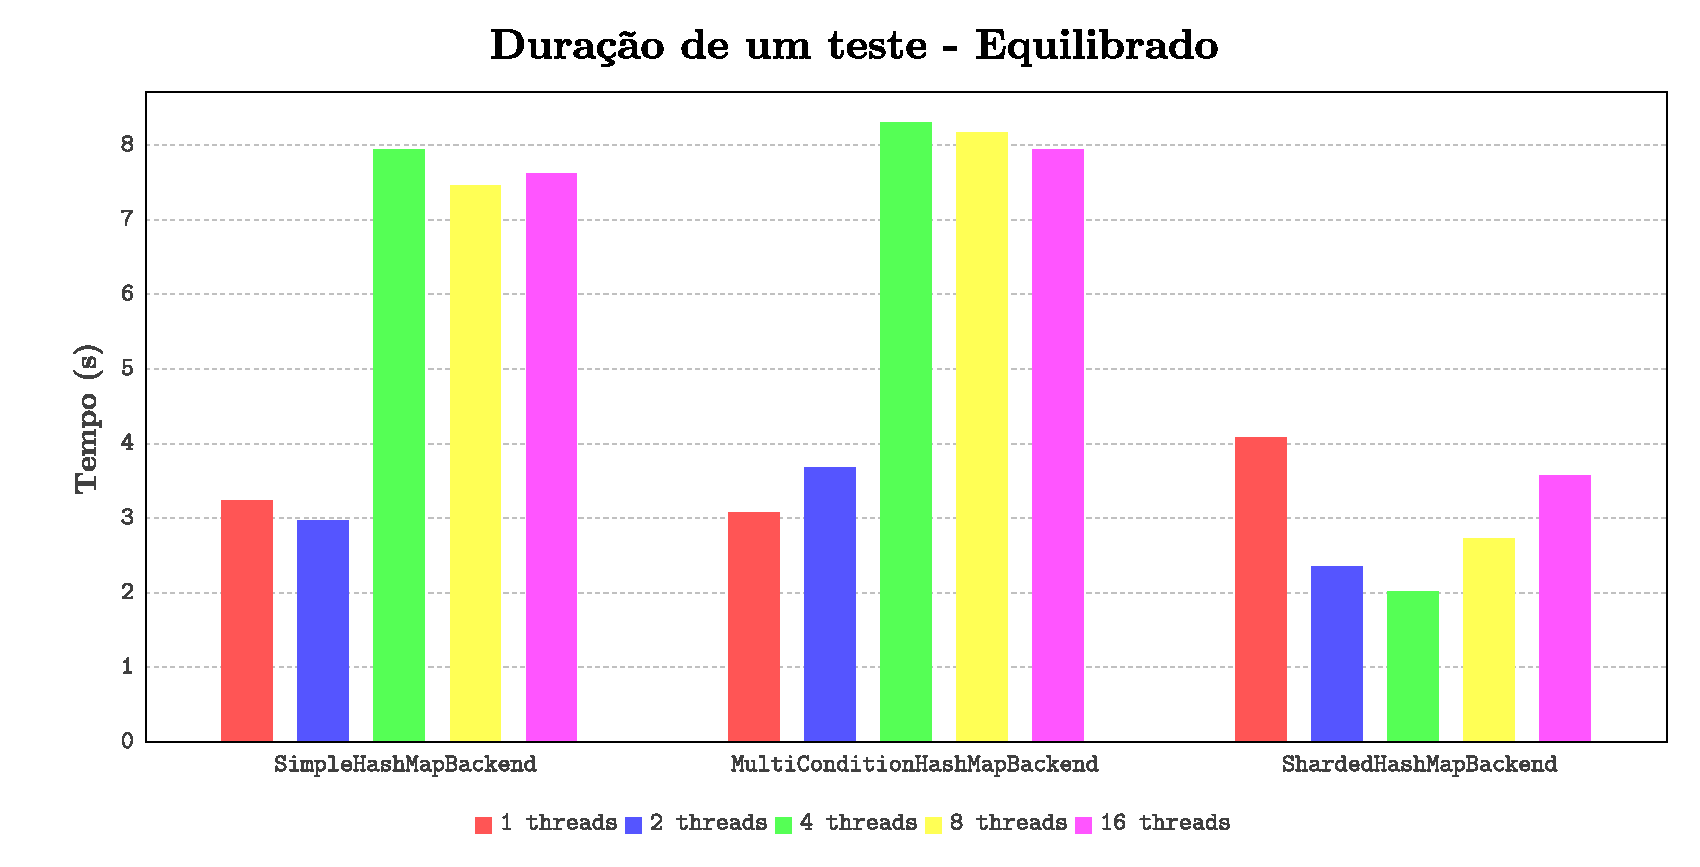
\includegraphics[width=0.45\textwidth]{autogen/Equilibrado.eps}
    \end{longtable}
    \caption{Duração dos testes dependendo do \emph{benchmark}, \emph{backend} e número de
        \emph{threads} escolhidos.}
    \label{time-graphs}
\end{figure}

\section{Conclusão}

\section{Bibliografia}
\def\refname{}
\vspace{-1.5cm}
\begin{thebibliography}{9}
    \bibitem{apache-commons-math}
        The Apache Software Foundation. "Commons Math: The Apache Commons Mathematics Library."{},
        Apache Commons. Accessed: Dec. 20, 2024. [Online.] Available:
        \url{https://commons.apache.org/proper/commons-math/}

    \bibitem{jfreechart}
        D. Gilbert. "Welcome To JFreeChart!."{}, JFreeChart. Accessed: Dec. 20, 2024. [Online.]
        Available: \url{https://www.jfree.org/jfreechart/}

    \bibitem{apache-xml-graphics}
        The Apache Software Foundation. "Apache FOP."{} The Apache XML Graphics Project. Accessed:
        Dec. 20, 2024. [Online.] Available: \url{https://xmlgraphics.apache.org/fop/}
\end{thebibliography}

\section{Anexos}

\subsection{Características do \emph{benchmarks}}
\label{benckmark-description}

\begin{table}[H]
    \begin{center}
        \begin{tabular}{|m{5cm}|c|c|c|}
            \hline & Maioritariamente leituras & Equilibrado & Equilibrado c/ \texttt{getWhen} \\

            \hline Número de chaves         & \multicolumn{3}{c|}{1024}         \\
            \hline Número de valores        & \multicolumn{3}{c|}{1024}         \\
            \hline Comprimento de uma chave & \multicolumn{3}{c|}{8 caracteres} \\
            \hline Comprimento de um valor  & \multicolumn{3}{c|}{8 octetos}    \\

            \hline Percentagem de \texttt{put}s      & 5  & 25 & 25 \\
            \hline Percentagem de \texttt{get}s      & 70 & 25 & 20 \\
            \hline Percentagem de \texttt{multiPut}s & 0  & 25 & 25 \\
            \hline Percentagem de \texttt{multiGet}s & 25 & 25 & 25 \\
            \hline Percentagem de \texttt{getWhen}s  & 0  & 0  & 5  \\

            \hline Distribuição de chaves  & \multicolumn{3}{c|}{Uniforme} \\
            \hline Distribuição de valores & \multicolumn{3}{c|}{Uniforme} \\
            \hline Distribuição de número de chaves em operações multi &
                \multicolumn{3}{c|}{Uniforme entre 2 e 4, inclusive} \\

            \hline Número de operações & \multicolumn{2}{c|}{8 milhões} & 1 milhão\footnotemark \\
            \hline Tamanho de um bloco & \multicolumn{3}{c|}{4096} \\
            \hline
        \end{tabular}
    \end{center}

    \caption{Características dos \emph{benchmarks} concebidos.}
\end{table}

\footnotetext{
    Devido à \emph{thread} de desbloqueio de operações \texttt{getWhen}, o teste seria muito
    demorado caso fossem executadas 8 milhões de operações.
}

Os três \emph{backends} foram testados, sendo que o \texttt{ShardedHashMapBackend} foi inicializado
com 64 \emph{shards} e não foi sujeito ao \emph{benchmark} "Equilibrado c/ \texttt{getWhen}"{}.

\subsection{\emph{Hardware} e \emph{software} utilizados para a execução dos \emph{benchmarks}}
\label{hardware-software-description}

\begin{table}[H]
    \begin{center}
        \begin{tabular}{|c|c|}
            \hline Processador       & Intel Core i3-7100 3.9 GHz  \\
            \hline Memória           & 8 GiB DDR4 2400 MT/s        \\
            \hline Sistema Operativo & Linux 6.11.5                \\
            \hline JRE               & OpenJDK 21.0.5              \\
            \hline
        \end{tabular}
    \end{center}

    \caption{\emph{Hardware} e \emph{software} utilizados para a execução dos \emph{benchmarks}.}
    \label{hardware-software}
\end{table}

\end{document}
